\chapter{Example Chapter Title}
\label{chap:example_chapter}

This is an example chapter with some text. You don't need to name your chapters as "Chapter 1", "Chapter 2", etc. Rather, following the practice of \LaTeX, it is better to name and label your chapters descriptively. And the numbering of the chapters will be done automatically when you include them in your \verb|main.tex| file. If you want to include a new chapter in your document, create a \verb|chapter_name.tex| file in the \verb|Chapters| directory and include it in your \verb|main.tex| file using the \verb|\include{./Chapters/chapter_name}| command.

You can include figures, tables, and equations in your chapters. You can also include subfigures and subtables. I selected a few texts in the formatting guidelines and provided some examples below.

\section{Headings and Subheadings}
\label{sec:headings}

Graduate Services does not set specific style standards for the format of chapter headings and subheadings except for font size—font size for all headings should be the same as the body of your text (if your text is 12 pt., then your headings must also be 12 pt.). There is a suggested format for heading style in the required templates provided by Graduate Services. Students should refer to the standards set by their department's choice of style manual. Regardless of the formatting style chosen, Graduate Services does require that the style be applied consistently to all headings and subheadings throughout the document. 


\section{Journal Articles Used as Chapters}
\label{sec:journal_articles}
In some departments, theses or dissertations may include as chapters, articles that have been or will be submitted to scholarly journals. This is an acceptable style; however, you must be listed as an author with clear evidence of your intellectual leadership in the publication. How this is represented varies across disciplines; it may take the form of sole authorship, lead authorship, or corresponding authorship, and the publication may not be included in any other individual's thesis or dissertation, whether at GSU or any other institution. A brief statement should be included at the conclusion of the chapter describing the intellectual leadership and any other research roles played by the student in developing and publishing the research. 
 
In addition, the general formatting requirements listed above also apply to articles used as chapters. You MUST apply a consistent style in your font, headings, subheadings, tables and figures throughout each article used as a chapter, as well as your general introduction and conclusion. Evidence of permission to use articles which have been published or accepted for publication must be included. It is the student's responsibility to secure such copyright releases prior to submitting the thesis/dissertation to Graduate Services. Graduate Services will accept a letter of permission or an e-mail from the publisher. Graduate Services will not accept a thesis or dissertation for the final submission unless all copyright releases are on file (articles that have yet to be submitted or are under review do not need copyright releases.) 





\section{Reference Examples}
\label{sec:reference_examples}

And as an example of citing things, here is the \TeX book by Knuth in 1986~\cite{knuth1986texbook}. See \verb|bibliography.bib| for adding reference items. Format of the reference entries should be according to your department or discipline's choice of style manual. That said, you do have the option to create references or works cited pages for each chapter rather than a large comprehensive list of references.


\section{Figures and Tables}
\label{sec:figures_tables}

Sample Figures and Tables below.

\begin{figure*}[H]
	\centering
	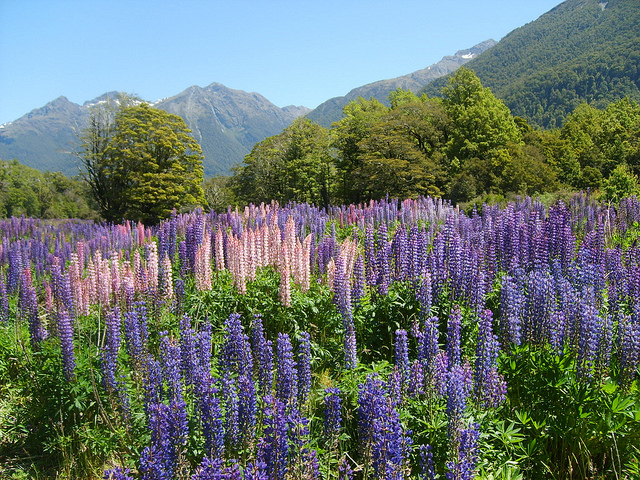
\includegraphics[width=0.7\textwidth]{./Plots/nature.jpg}
	\caption{An individual figure!}
\end{figure*}
        
\begin{figure*}[H]
	\centering
	\subfloat[\label{fig:HD8538_ellplot}]{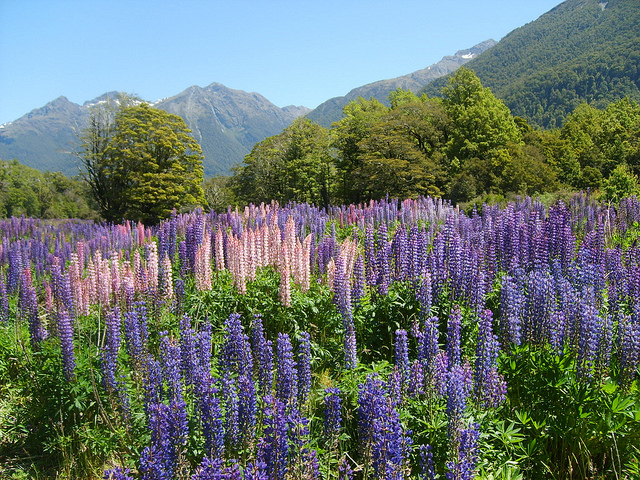
\includegraphics[width=.4\textwidth]{./Plots/nature.jpg}} 
	\subfloat[\label{fig:HD8538_phot}]{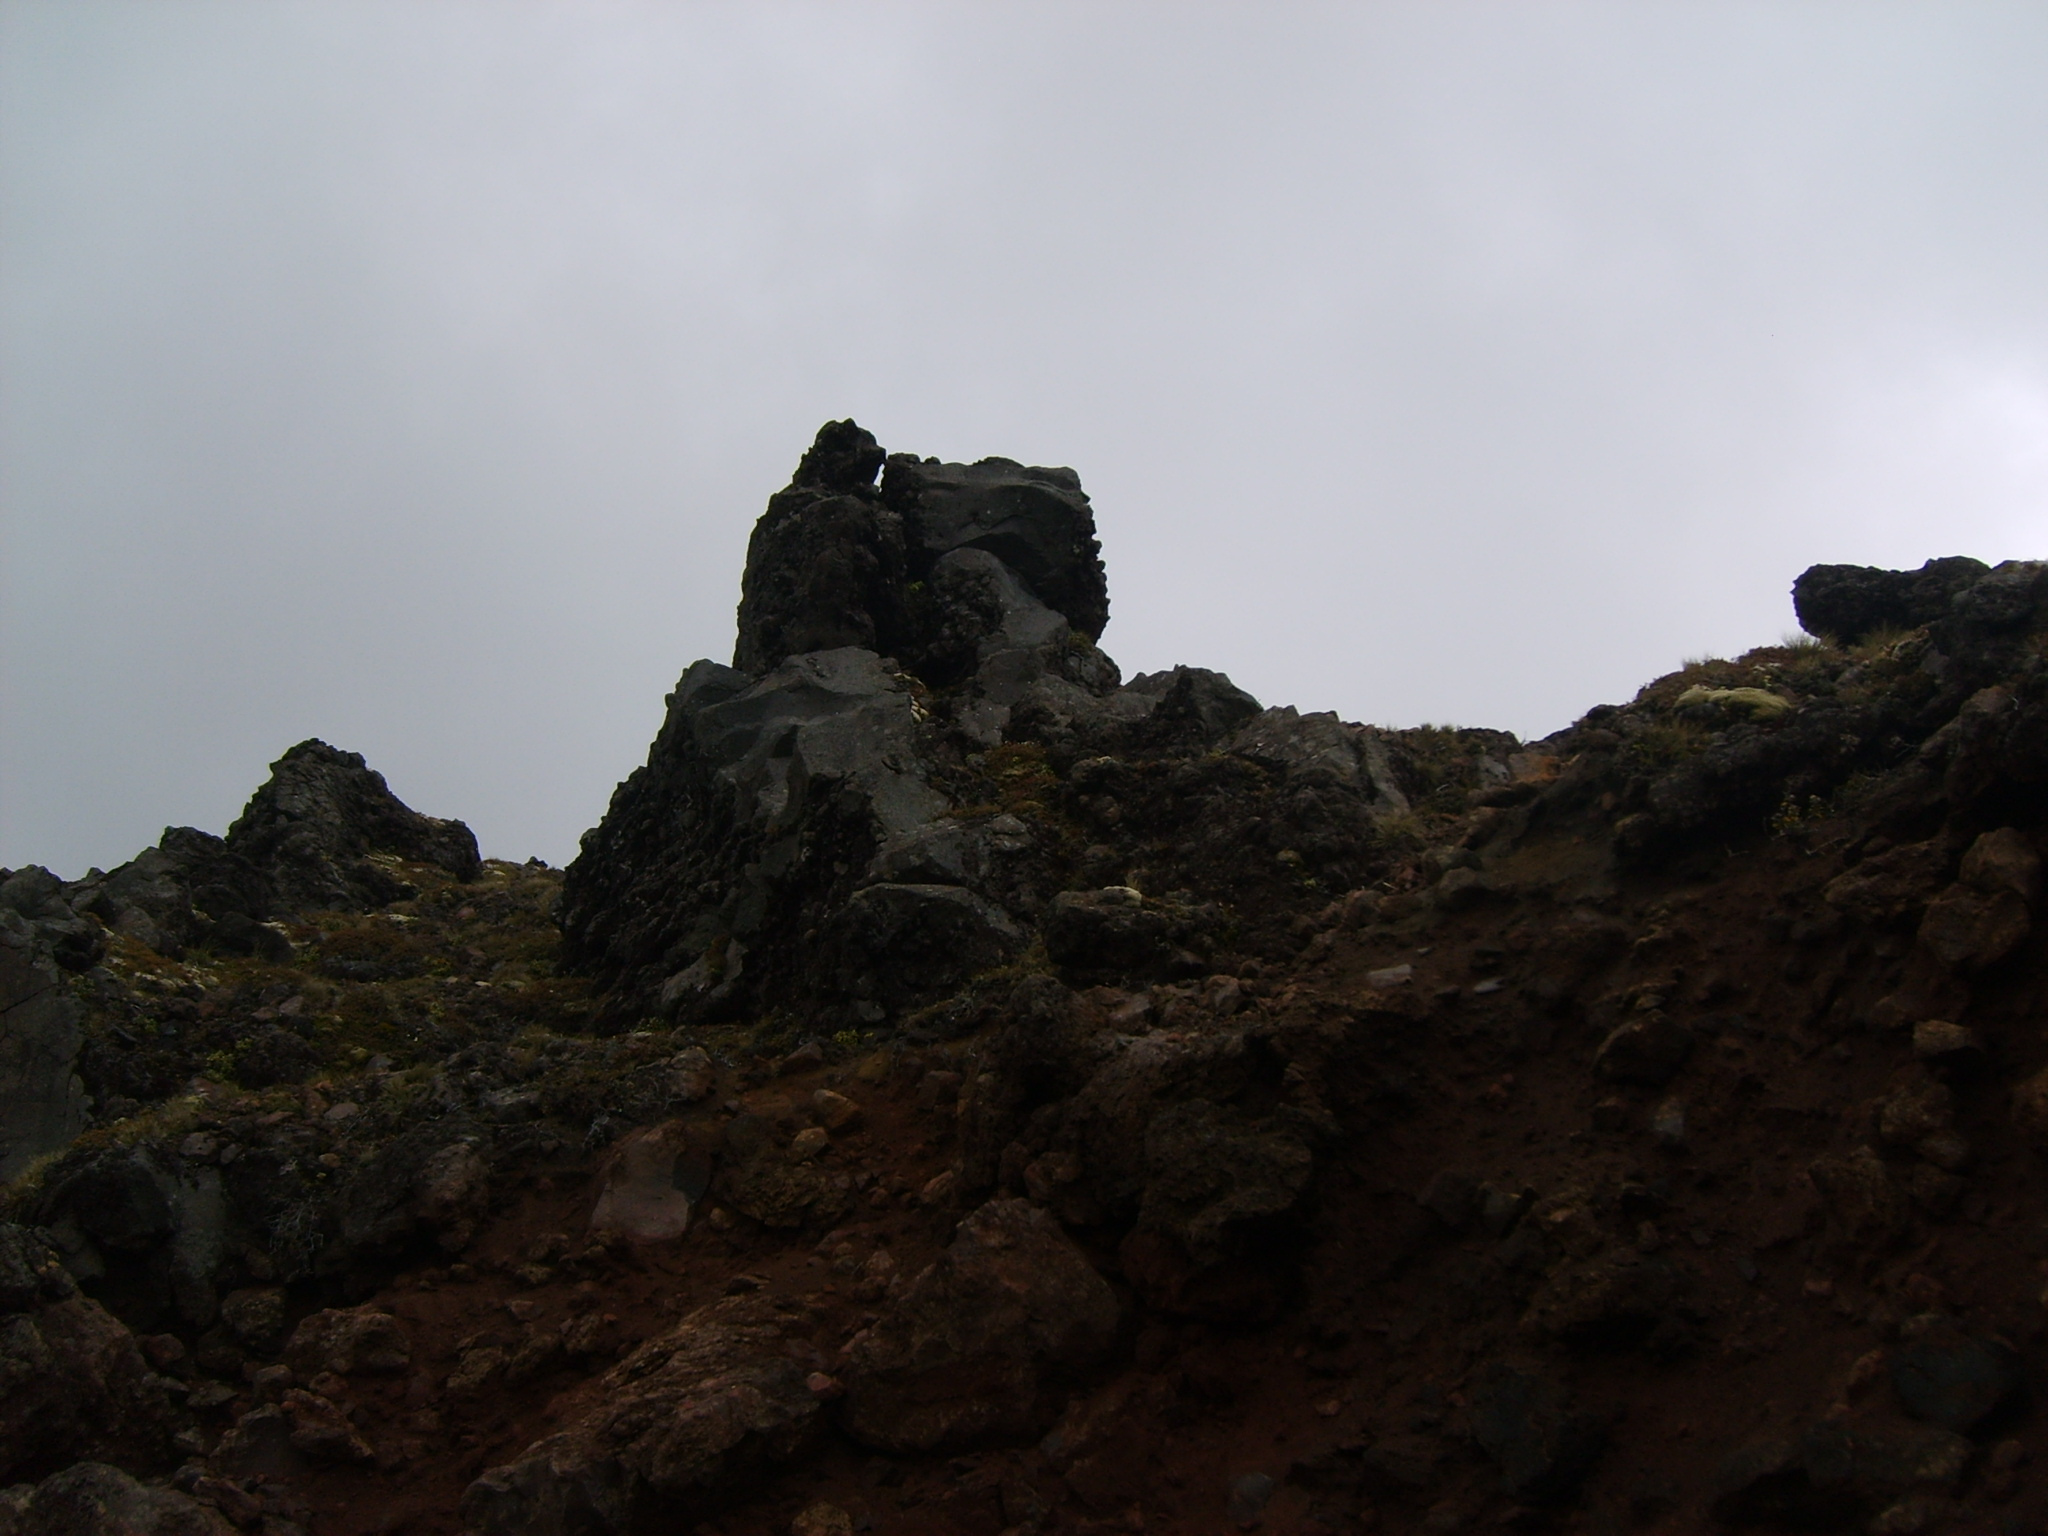
\includegraphics[width=.4\textwidth]{./Plots/rocks.jpg}} \\
	\subfloat[\label{fig:HD8538_vis}]{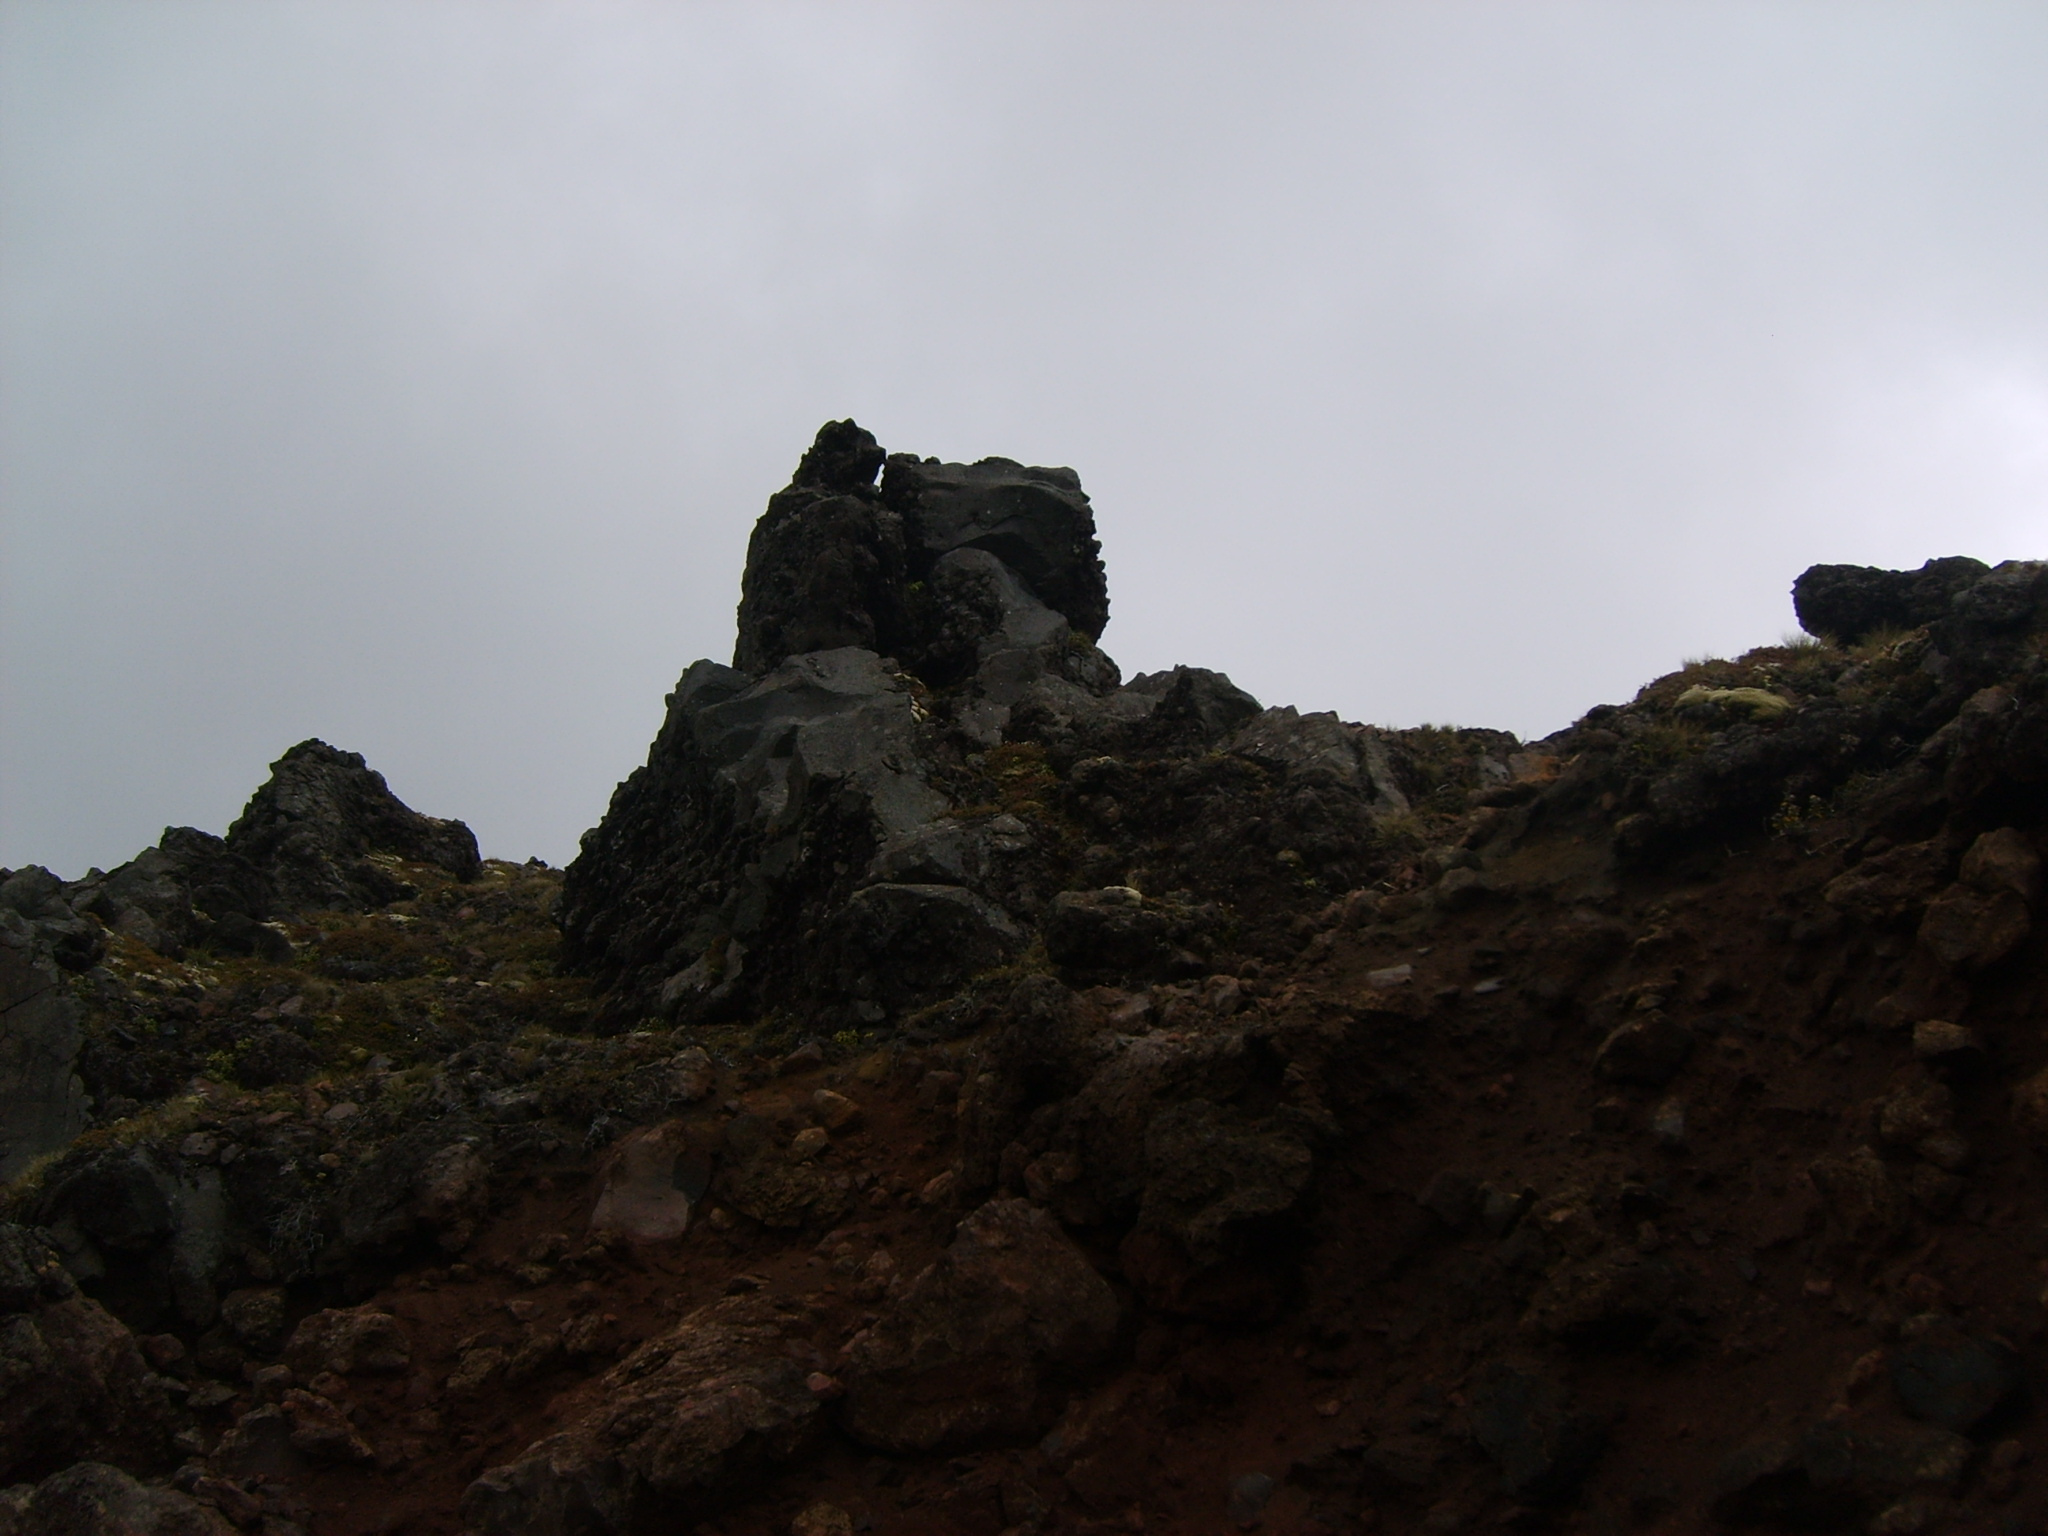
\includegraphics[width=.4\textwidth]{./Plots/rocks.jpg}}
	\subfloat[\label{fig:HD8538_HRD}]{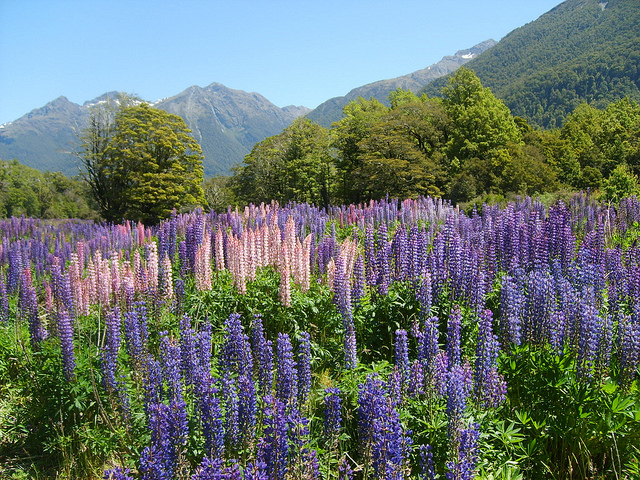
\includegraphics[width=.4\textwidth]{./Plots/nature.jpg}}
	\caption{Multiple figures!}
\end{figure*}

You can have a table like this:
\begin{table}[H]
	\centering
	\label{tab:simple_table}
	\caption{A simple table}
	\begin{tabular}{|c|c|c|}
		\hline
		\textbf{ID} & \textbf{Name} & \textbf{Course} \\
		\hline
		1 & John Doe & Mathematics \\
		2 & Jane Smith & Physics \\
		3 & Mary Johnson & Chemistry \\
		\hline
	\end{tabular}
\end{table}

You can also include a wide table like this:

\begin{landscape}
\begin{longtable}{cccccccccccccc}
\label{tab:wide_table_example}\\
\caption{An example of very large horizontal table}\\
\hline\endhead  % header material
\hline\endfoot  % footer material
\hline
\textbf{ID} & \textbf{Name} & \textbf{Age} & \textbf{Email} & \textbf{Phone} & \textbf{Major} & \textbf{Grade} & \textbf{Comments} \\
\hline
1 & John Doe & 20 & johndoe@example.com & 123-456-7890 & Mathematics & A & Excellent work \\

2 & Jane Smith & 22 & janesmith@example.com & 234-567-8901 & Physics & B & Good understanding \\

3 & Mary Johnson & 21 & maryjohnson@example.com & 345-678-9012 & Chemistry & A & Outstanding performance \\

4 & James Brown & 23 & jamesbrown@example.com & 456-789-0123 & Biology & C & Needs improvement \\

5 & Patricia Davis & 20 & patriciadavis@example.com & 567-890-1234 & English & B & Well done \\

6 & Robert Miller & 22 & robertmiller@example.com & 678-901-2345 & History & A & Excellent analysis \\

7 & Jennifer Wilson & 21 & jenniferwilson@example.com & 789-012-3456 & Geography & B & Good research \\

8 & Michael Moore & 23 & michaelmoore@example.com & 890-123-4567 & Computer Science & A & Great coding skills \\

9 & Linda Taylor & 20 & lindataylor@example.com & 901-234-5678 & Art & C & More practice needed \\

10 & William Anderson & 22 & williamanderson@example.com & 012-345-6789 & Music & B & Good performance \\
\hline
\end{longtable}
\end{landscape}


\section{Examples and Code Snippets}

Here is an example of code snippet:
\begin{code}
	print("Hello World!")
	for i in range(10):
		print(i)
\end{code}

If you want some example text, here is some:
\begin{example}
	Your example here
\end{example}